
%%1. The methodology proposed is not clearly explained in Sections 4 and 5 of the paper.
%%2. The presentation of the paper can be substantially improved including the English in the paper.
%%3. The motivation and problems statement is not good. Please, reinforce those section by introducing problems in the real world with references. Moreover, clarify the problems and your solutions with contribution in the introduction section.



\documentclass[AMA,STIX1COL]{WileyNJD-v2}
\usepackage{graphicx}
\usepackage[justification=centering]{caption}
\usepackage{CJK}
\usepackage[top=2cm, bottom=2cm, left=2cm, right=2cm]{geometry}
\usepackage{algorithmicx}
\usepackage{algpseudocode}
\usepackage{amsmath}
\usepackage{xcolor}%???????  
\usepackage{colortbl,booktabs}%?????????*rule  
\usepackage{caption}
\usepackage{subfigure}
 \usepackage{verbatim}
 \usepackage{pgfplots}
\usepackage{tikz}    
\usetikzlibrary{arrows,shapes,chains}  
%%\articletype{Article Type}%

\received{15 May 2018}
%\revised{6 June 2016}
%\accepted{6 June 2016}

\raggedbottom

\begin{document}

\title{A Node Backup Algorithm for Fault Cascade degradation in Virtualization Power Communication Network}

\author[1]{Lanlan Rui}

\author[2]{Zhen Xia}

\author[3]{Xuesong Qiu}

\author[4]{Peng Yu}



\address[1]{\orgname{State Key Laboratory of Networking and Switching Technology Beijing University of Posts and Telecommunications}, \orgaddress{\state{Beijing}, \country{China}}}

\address[2]{\orgname{State Key Laboratory of Networking and Switching Technology Beijing University of Posts and Telecommunications}, \orgaddress{\state{Beijing}, \country{China}}}

\address[3]{ \orgname{State Key Laboratory of Networking and Switching Technology Beijing University of Posts and Telecommunications}, \orgaddress{\state{Beijing}, \country{China}}}

\address[4]{ \orgname{State Key Laboratory of Networking and Switching Technology Beijing University of Posts and Telecommunications}, \orgaddress{\state{Beijing}, \country{China}}}

\corres{Lanlan Rui, \email{llrui@bupt.edu.cn}}

\presentaddress{State Key Laboratory of Networking and Switching Technology Beijing University of Posts and Telecommunication}

\abstract[Summary]{This paper examines fault cascade degradation in virtual power communication networks. To fulfill certain requirements (e.g., reasonable network design in a network virtualization (NV)environment), we propose a network optimization algorithm called the primary nodes group algorithm (PNGA), which is based on the complex network approach. The main goal of PNGA is promoting the overall robustness of the network. 

\par In the simulation experiment, we analyze the network modeling and topological characteristics of a three-tier power grid under NV. Furthermore, we use a degree sorting algorithm (which is widely used in power grids)as a control group. Under different attack strategies, we analyze the performance of different algorithms and the states of fault generation. The results of these simulations demonstrates that PNGA has superior fault suppression when compared with other algorithms.}

\keywords{ Power communication network, network virtualization, cascade fault, backup optimization algorithm, complex network}

\jnlcitation{}

\maketitle


\pgfplotsset{every axis legend/.style={%
cells={anchor=west},
inner xsep=3pt,inner ysep=2pt,nodes={inner sep=2pt,text depth=0.15em},
anchor=north east,%
shape=rectangle,%
%fill=white,%
draw=black,
at={(0.98,0.98)}
}}


\section{Introduction}\label{sec1}
\par In recent years, intelligent power systems have developed rapidly, making existing power grids more dependent on the reliable operation of power communication networks [1-3]. Moreover, unstable communication subsystems have historically played a negative role in major power blackouts such as the 2003 North American blackout [5], the Italian power outage, and the 2011 Mexico blackout [7]. During the Italian blackout (September 28th, 2003), the European interconnected grid faced a series of outages. In addition, the interconnecting lines were already overloaded. This incident affected approximately 45 million people with full restoration of service taking 19 hours. The consequences of a large blackouts are very serious [4]; therefore, studying the vulnerability and improving the robustness of power communication networks is a crucial research domain. Power communication networks are typically complex in structure [6]. Thus, we use complex network approach to analyze and study specific fault tolerance problems in this paper.

\par Severe phenomena have been reported in power communication networks [6], and some of these incidents are not detectable by conventional protection schemes. Thus, network administrators must understand the structures of power communication networks and the power grids they serve. Due to the high cost of refactoring actual networks, network virtualization is widely used in power communication network structures. Network virtualization deals with the virtualization of network functions usually performed by dedicated hardware devices. Both industry and academia are taking advantage of this technique to drive innovation and provide flexibility in network management [7]. In addition, virtualization provides network managers with the flexibility to control the working state of each node regardless of specific network environments or high optimization costs.
\par By analyzing the complexity and high coupling of grid structures and the causes of faults, this paper determines the essential characteristics of a reliable power communication network. Combined with the design requirements of a given communication network, this paper transforms a real-world situation into a minimum connected dominating set (MCDS). In tandem with the MCDS method, we propose PNGA to replace the digital signature algorithm (DSA), thereby examining the tolerance of each node in the virtual backbone network to improve robustness. Following this, the simulation experiments of the backup optimization algorithm are performed. By comparing the different algorithms, we confirm the efficacy of our proposed method. Finally, we present our summary, conclusions, proposals for future work.

\par The main contributions of this paper are as follows: (1) A network-optimization scheme based in an NV environment is proposed to promote the robustness of power communication networks against the failures; (2) A coupled smart grid model is designed to describe the problem space. (3) The optimization algorithms for the primary node groups (based on the coupled model)are provided.
\section{Introduction of Architecture}\label{sec1}

\par In NV, a network is divided into the substrate network (SN) and virtual network (VN) [7]. The roles in a network virtualization model include the infrastructure provider (InP) and service providers (SP). The SP combines the functions that the VN provides to the outside world into services (Fig.1). The SN contains specific network components provided by the InP, such as the power communication network and the power grid [8]. NV management(NVMA) is responsible for resource management and network coordination. The algorithms in this paper run on the NVMA layer, which arranges and optimizes the internal power communication network of the VN. Unless otherwise specified, any network structures referred to later in this paper are within the VN.
\begin{figure}[htbp]
\centering
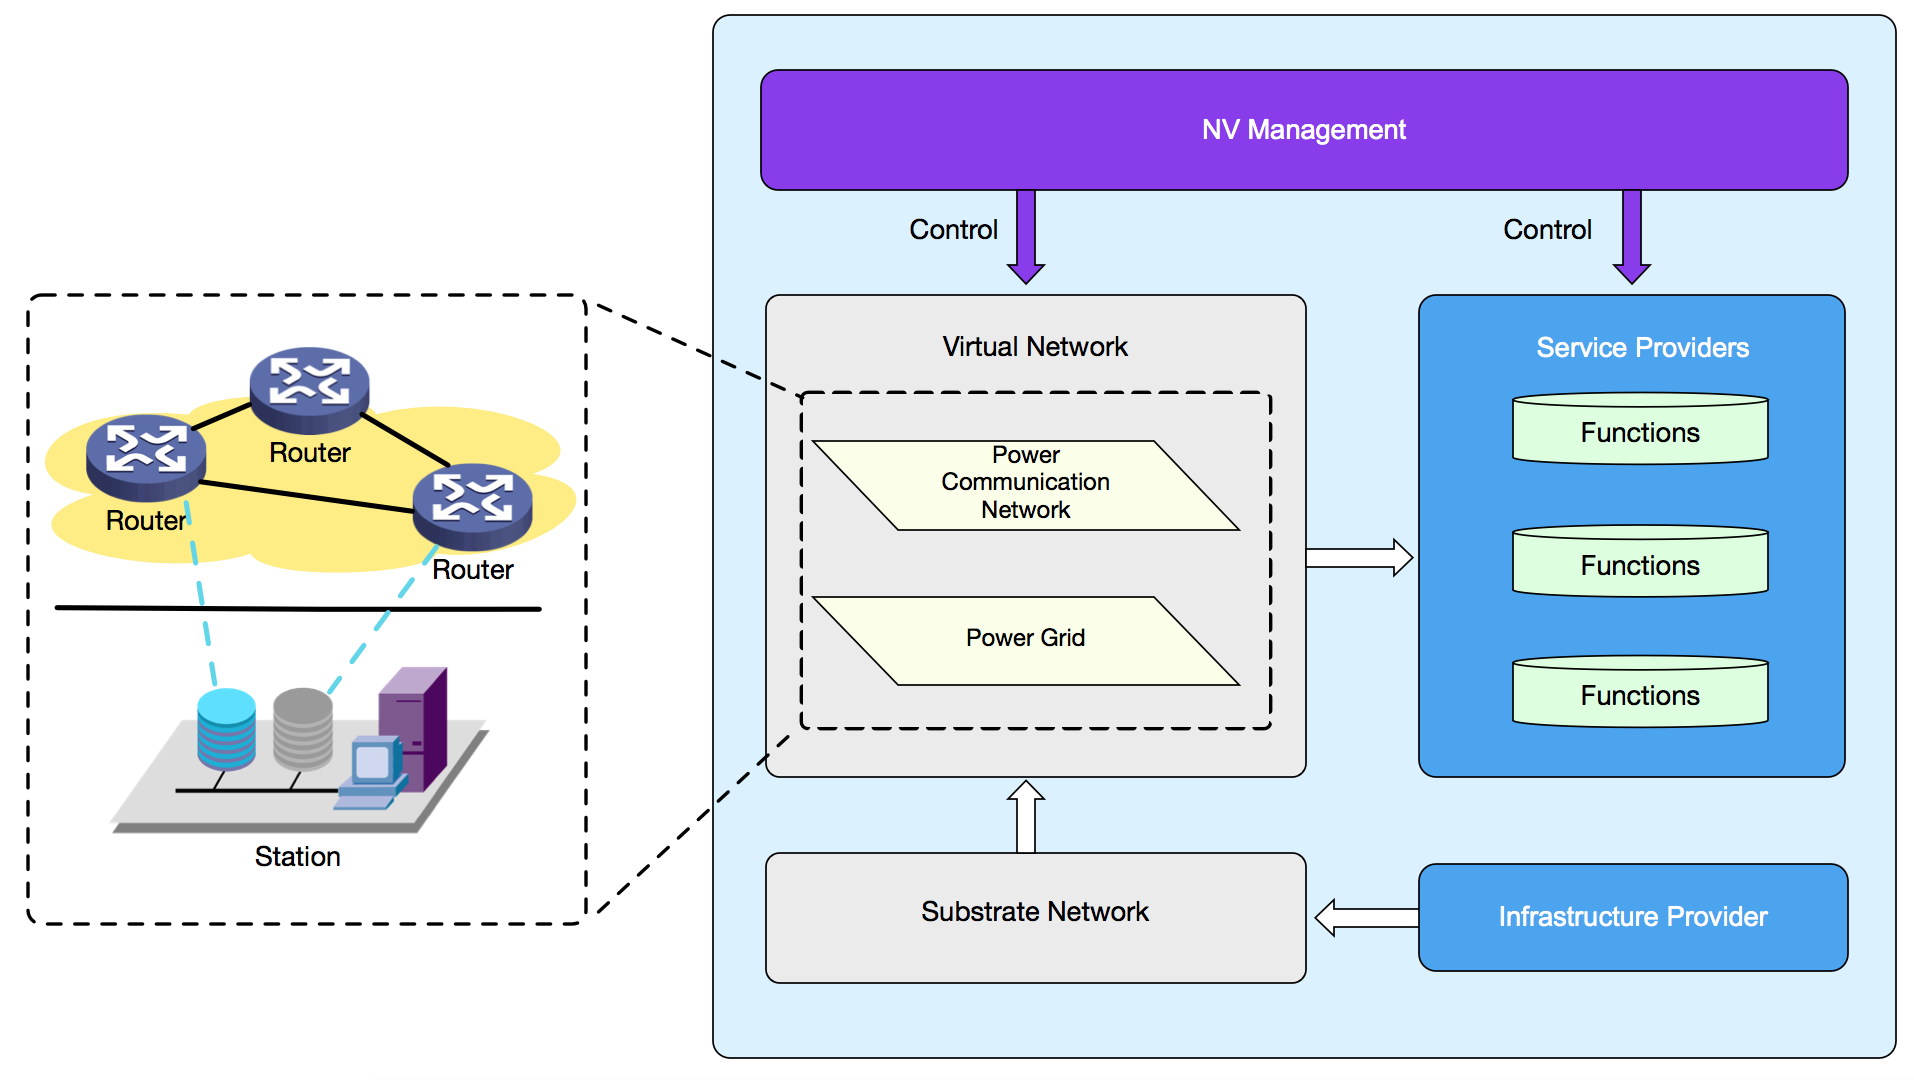
\includegraphics [width=6.5in]{NFV-1}
\caption{The architecture of the virtual power communication network}
\label{NV}
\end{figure}
\section{Related works}\label{sec2}
\par Despite all its benefits, NV presents many challenges (such as small NV deployments, performance issues, and NVMA-related issues) [8]. The project in [9] provides an architecture for deploying and managing virtual network functions in a cloud environment using open standards. Moreover, the TeNOR orchestration platform [10] focuses on the automated deployment and configuration of services and resource sharing optimization. Likewise, Maestro [11] considers the internal composition of services for selecting an optimal deployment setup on wireless networks.

\par At present, most power sub-networks are similar to scale-free and small world networks. In [12], the vulnerabilities of these two networks is aptly illustrated. Given these vulnerabilities, there are two main research directions to consider. The first is based on complex network theory. Here, the vulnerability of a power communication network is evaluated from the view of network efficiency [13]. In [14], the topology evolution process of a synchronous digital hierarchy (SDH) optical fiber communication network was studied. Finally, in [15], a static and dynamic vulnerability assessment method for information networks was proposed based on complex network theory. The second idea is to focus on communication services. This approach improves the robustness of the communication networks by updating equipment and establishing a reasonable security assessment system. In [15], the authors proposed the concept of business risk balanced with rational arrangements for the communication network business channels and modes of operation.

\par In [16], a service routing optimization algorithm based on the reliability of power communication networks was proposed. However, this approach did not account for the particularity of the grid structure. In this algorithm, we simplified the power communication network into a simple routing topology in the services layer.

\par Topology is the most natural and essential attribute of a power communication network. The efficient transmission of communication services is based on the reliable physical network. The power communications business is extensive and complex. Moreover, vulnerable nodes in the network are more likely to be targeted. Based on complex network theory, the inherent structural vulnerabilities of a power communication network can be identified and targeted protection strategies can be implemented.

\par Although some scholars have proposed the idea of adding multiple physically independent topologies to improve network vulnerability [17], there is a lack of comparative research on various backup strategies; their effectiveness has not yet been demonstrated in actual power communication networks. The topological structures of primary power networks have been extensively studied; thus, it is necessary to continue with the thorough analysis of power communication network topology, and compare the validity of existing backup strategies.

\par From the perspective of an entire power grid, this article combines the highly coupled structure of power grids and the physical requirements of the communication cables and derives a backup optimization algorithm for power communication networks.



\section{Smart Grid}
\par First, we analyze the structures and fault generation and processing mechanisms of an entire smart grid to draw the necessary conclusions and produce the required mathematical models related to the optimization of communication network backup.

\par Smart grids comprise a power system and communications network. The routers in the communication network require power from the power system, and the power system needs transmission decision information from the communication network.  The unique nature of this coupling has attracted the attention of many researchers. Some researchers have explored the coupling relationship between mutually beneficial and heterogeneous networks [19], and many have studied the coupling systems in variable electronic stations equipped with advanced intelligent devices such as intelligent electronic devices (IEDs) and flexible AC transmission systems (FACTS) [18].
\par However, most current studies ignore the impact of internal node interactions [20]. In addition, network managers often pay too much attention to specific business assignments. Thus, a smart grid relies on the overall network of interconnected power networks and communication networks. Hence, in the process of data communication and information exchange, the power network and the nodes in the communication network interact.
\par In this section, a mathematical model is created for the grid to understand the interaction between the power nodes and communication nodes in the grid and the process of fault generation. Table \ref{Definition} shows the definition of mathematical functions and parameters. 
\begin{table}[htbp]
\centering
\caption{Definition}
\label{Definition}
\begin{tabular}{@{}
>{\columncolor[HTML]{FFFFFF}}c 
>{\columncolor[HTML]{FFFFFF}}c @{}}
\toprule
Definition & Description                                                                                                                                           \\ \midrule
N    &   the network size,              \\ \midrule
K          & the average degree  \\ \midrule
p          & the connection probability     \\ \midrule
L(p)          & the average path length of the small world model                                                                                                                                 \\ \midrule
C(p)       & the  degree  of  network  grouping                                                                                                      \\ \midrule
G   &  the network \\ \midrule
Q(G)/QP(G)          &  the network evaluation function \\ \midrule
R   & the ratio of the number of nodes that were  attacked  before  the  network  crashes  to  the  total  number  of  nodes                                                                                                       \\ \midrule

Rc     & the threshold for node removal                                                                                                \\ \midrule
Z     & the nodewith the largest degree of network                                                                                                \\ \midrule
m     & the node with the smallest degree of the network                                                                                               \\ \midrule
H     & the degree distribution entropy                                                                                               \\ \midrule
X        &  the  sampling point                                                                                                           \\ \midrule
W     & the percentage of workable nodes                                                                                                           \\ \bottomrule


\end{tabular}
\end{table}
\subsection{The basic concept of complex network of power communication}
\par Although most power communication networks are large, there is a rather short path between each pair of nodes. This reflects both the small number of interrelationships and the ability to connect to the world. So far, there is no precise expression to analyze the average path length of the small world model. However, we used renormalization group analysis to produce equation (1)[20], where N denotes the network size, K denotes the average degree, and p indicates the connection probability.

\begin{equation} 
L\left ( p \right )= \frac{2N}{K}f\left ( \frac{NKp}{2} \right )
\end{equation}

The expression of the f function is equation (2), as follows:

\begin{equation} 
f\left ( x \right )= \left\{\begin{matrix}
constant, x\ll 1\\ \\
\left ( \ln x \right )/{x},        x\gg  1
\end{matrix}\right.
\end{equation}

\par At present, many academics use an averaging method to give the approximate expression of the above equation as follows:

\begin{equation} 
f\left ( x \right )\approx \frac{1}{2\sqrt{x^{2}+2x}}\arctan h\sqrt{\frac{x}{x+2}}
\end{equation}

Agglomeration indicates the degree of network grouping, and the concept of connected groups reflects the distribution and interrelated status of small networks. Since the aggregation coefficient is a function of the connection probability p, the corresponding aggregation factor when the value of p is 0 is as follows:

\begin{equation} 
C\left ( 0 \right ) = \frac{3}{2}\left ( \frac{K}{2} - 1 \right )/\left (K-1  \right )
\end{equation}

\begin{equation} 
C\left ( p \right ) = \frac{3\left(K-2 \right )}{4\left (K-1  \right )}\left (1-p  \right )^{3}
\end{equation}

Thus, we can approximate that:

\begin{equation} 
C\left ( p \right ) = C\left ( 0 \right )  \left (1-p  \right )^{3}
\end{equation}

\subsection{Robustness Measure}
\par This section describes two network evaluation functions: Q(G) and QP(G).
\subsubsection{Q(G)}

\par In the study of network robustness, there are many concepts concerning topology attributes. Moreover, the most intuitive way to show the current state of a network is the size of the largest connected subgraph. It is clear that when the degree of network collapse reaches a certain threshold, the nodes of the network are split into separate small subgraphs, which can carry too little information and cannot restore the performance of the entire network. Therefore, quantitative analysis of network attacks is of critical importance. 
\par The critical point removal ratio is defined as follows: When the nodes in a network are attacked, the ratio of the number of nodes that were attacked before the network crashes to the total number of nodes is denoted by R, which is the critical point removal ratio. When the network is facing external attacks, Rc is the threshold for node removal. The percentage R of nodes are removed, and when R $>$ Rc, the network crashes into many independent small connected subgraphs. When R $<$ Rc, there is a complete connected area in the network.

\par Considering that both the distribution of nodes in the network and the amount of the information in the communication network are expressed in a probabilistic form, we extend the concept of entropy in information theory to complex networks. According to the definition of information, we define the degree distribution entropy in complex networks as follows: Z is the node with the largest degree in the network and m is the node with the smallest degree in the network. 

\begin{equation} 
H=-\sum_{k=1}^{N-1}p\left ( k \right ) \mathbf{log} (p\left ( k \right ))
\end{equation}

\begin{equation} 
p\left ( k \right )=ck^{-a}, k = m, m+1, ..  ,Z
\end{equation}

\par When the network scale is relatively large, we can perform the following analysis:

\begin{equation} 
H=-\sum_{k=1}^{N-1}p\left ( k \right ) \mathbf{log} (p\left ( k \right )) \\ \\
=-\int_{m}^{Z}p\left ( k \right ) \mathbf{log} (p\left ( k \right ))\mathrm{d} k
\end{equation}

\begin{equation} 
H=-\int_{m}^{Z}ck^{-a}\mathbf{log} (ck^{-a})\mathrm{d} k
\end{equation}

\begin{equation} 
H=-\int_{m}^{Z}ck^{-a}\left ( \mathbf{log} c + \mathbf{log} (k^{-a})\right )\mathrm{d} k
\end{equation}
\begin{equation} 
H=-\left( \frac{c \mathbf{log}c }{1-a}k^{1-a } - \frac{ca}{1-a}\left( \mathbf{log}k\cdot k^{1-a} - \frac{1}{1-a}k^{1-a}  \right )\right )|_m^Z
\end{equation}
\par The value of Z is as follows:
\begin{equation} 
Z = mN^{\frac{1}{a-1}}
\end{equation}

\par The parameter c can be given by the following equation:


\begin{equation} 
1=\int_{m}^{\infty}p\left ( k \right )\mathrm{d} k=\int_{m}^{\infty}ck^{-a}\mathrm{d} k = \frac{c}{1-a}(-m^{1-a})
\end{equation}
\begin{equation}
c= (a-1)m^{a-1}
\end{equation}

\par Thus, we derive the following formula:

\begin{equation}
H(a,m,N)=\left ( \mathbf{log}\left ( \frac{a-1}{m} \right ) - \frac{a}{a-1} \right )(\frac{1}{N}-1)+\frac{a}{a-1}\frac{\mathbf{log}N}{N} 
\end{equation}


\par From the above equation we can conclude that the robustness of the network is related to the number of nodes in the network and the minimum value of the node degrees.


\par Thus, we can derive the function of the network for the anti-failure performance equation (7), where P represents the sampling point and W represents the percentage of workable nodes:

\begin{equation} 
q\left ( G \right )= \left (  \sum_{i=1}^{m}W_iX_i \right )/m
\end{equation}

In the normalization of the above formula, we introduce equation (8): 

\begin{equation} 
\theta (x)=\arctan \left ( x \right )\ast 2/\mathrm{Pi}
\end{equation}

The final function is as follows: ( C = 2 / Pi )

\begin{equation} 
Q\left ( G \right )= \theta (q\left ( G \right ))=\arctan \left (  \frac{ \sum_{i=1}^{m}W_iX_i}{m}  \right )\ast C \\
\end{equation}
\subsubsection{QP(G)}
\par QP (G) refers to the network evaluation function based on Q (G) in the production environment. 
\par Thus, Q (G) works well in the development environment and in part of the test environment. However, in the production environment, most of the network attack is inefficient and the network remains in normal working condition in most cases. Note that the assessment of the overall situation of the network and the analysis of the initial state of the network are equally important; QP (G) is used to describe this problem.
\par QP (G) is based on Q (G). The specific formula is as follows: We define the intermediate function D (S, G), S represents samples. 
\begin{equation} 
D\left (S, G\right )=\arctan \left (  \frac{ \sum_{i=1}^{S}W_iX_i}{S}  \right )\ast C \\  
\end{equation}
\par M represents the network samples, K is a subset of M and indicates the network samples at the beginning of the attack. Hence, Q(G) and QP(G) can be expressed as follows:
\begin{equation} 
Q\left (G \right ) = D\left (M, G \right )\\
\end{equation}
\begin{equation} 
QP (G) = D\left (K, G \right )
\end{equation}

\section{Coupled Model of Smart Grid}
\subsection{Coupled network model}
\par Intelligent power network systems are designed with great precision [20], allowing administrators to detect network failures promptly. This paper is based on the power fault propagation (PFP) model proposed in [21]; however, due to the complexity of the factors considered here, we use an optimized PFP model to describe our proposed system. This optimized model emphasizes the interaction of the network nodes and removes redundant parameters. We studied this model to discover hidden problems; the corresponding algorithm is then proposed.
\par This section outlines the modeling of the power network. For the convenience of presentation, G denotes a coupling network, R denotes a router, and S denotes a power plant. For a given power network, the degree of the power node V is the number of its neighbor nodes.

\par As shown in Fig. \ref{model}, the Ge icon indicates the control center. When a power system fails, the power plant generally reduces its load. The red line means power transmission. In general, Ge (the control center) is located in the city or town of the electrical authority, and routers are connected directly or indirectly to the control center via fiber.
\begin{figure}[htbp]
\centering
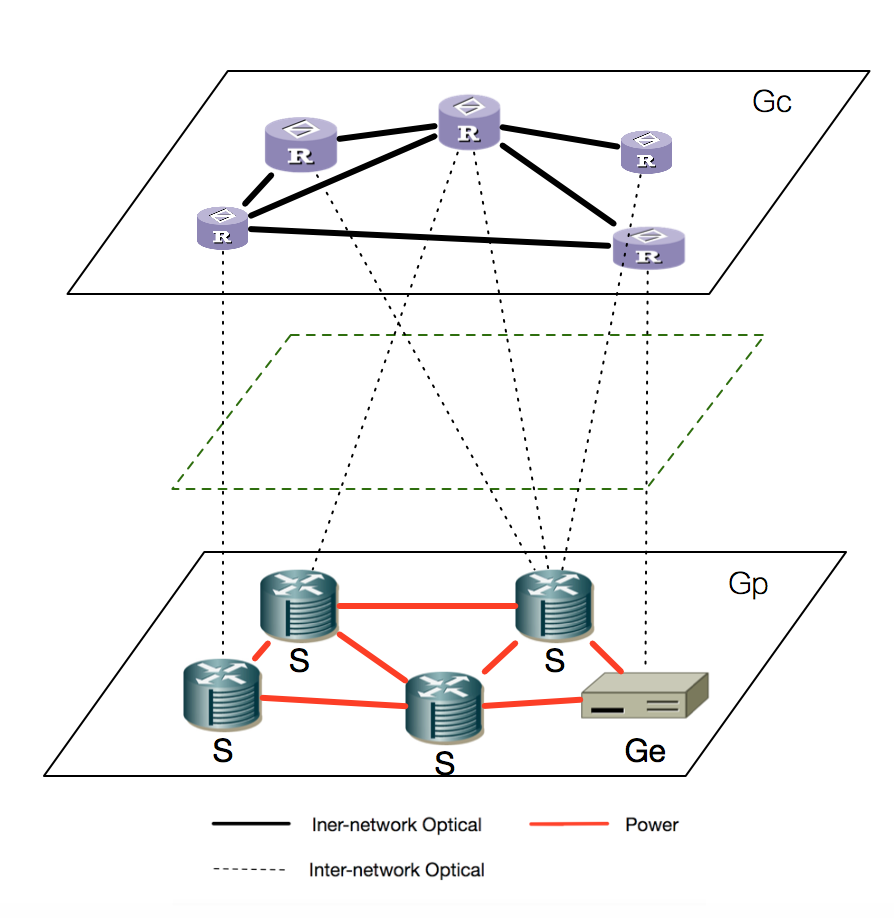
\includegraphics [width=4in]{2.png}
\caption{Coupled network model}
\label{model}
\end{figure}
\newpage
\par Given that Gp represents a power network and Gc represents a communication network, each graph has its own set of nodes and links; these are represented by V and E. The link between the two networks is denoted as Epc.
\subsection{Analysis of Power Grid Fault Handling Mechanism}
\par To precisely analyze the faults in the coupled network, this section defines the node failures explicitly. The node fault indication function of the optimized PFP model is defined as follows: When the substation fails, the value is 1. Otherwise, the value is 0:

\begin{equation} 
\delta (x)=\left\{\begin{matrix}
1, &  x=fail \\ 
0,&  x=work
\end{matrix}\right.
\end{equation}

\par The definition function is defined as follows:

\begin{equation} 
\forall v_{j}\in V^{c}, corr(v_{j})=\left \{v_{i} |(v_{i}, v_{j}) \in E^{pc}, v_{i}\in V^{p} \right \}
\end{equation}

\begin{equation} 
\forall v_{i}\in V^{p}, corr(v_{i})=\left \{v_{j} |(v_{i}, v_{j}) \in E^{pc}, v_{j}\in V^{c} \right \}
\end{equation}

\par According to the description of the grid fault handling mechanism in [22], the power failure process is as follows: When a substation fails, the node fault information is sent to the communication network. When the communication subnet receives the fault information, it will route power control commands to the power plant. 

\par We can assume that at least one power station Sj and a router Ri are faulty. Moreover, we can find the sumPath within the network. Otherwise, according to the fault handling mechanism of the power grid, this failure can be resolved by the network. 
\par In one case, assuming that Sj is directly connected to Ri, the sumPath is established. 
\par In another case, corr (Sj) is not connected to Ri. Thus, corr (Sj) can communicate directly with the power station, and the grid fault handling mechanism can resolve the problem; thus, we derive the sumPath. At the same time, the power station also belongs to the grid node, and we determine the finalPath. From the perspective of the communications network, the sPath is the key path. Thus:

\begin{equation} 
sumPath(S_{j}) = \{S_{j}, corr(S_{j})\} + \{R_{i}, R_{i+1},,,Ge\} + \{Ge,,,S_{j-1},S_{j}\}
\end{equation}

\begin{equation} 
sPath(S_{j}) = \{corr(S_{j}),R_{i}, R_{i+1},,,corr(Ge))
\end{equation}

\begin{equation} 
finalPath(S_{j}) = \{S_{j}\}+sPath + \{Ge,,,S_{j-1},S_{j}\}
\end{equation}

\section{Network Optimization}
\par As can be seen in the previous section, the critical path redundancy is the key to optimizing the communication network; the network structure must be modified. There are usually two redundant backup modes (redundancy for the edge and redundancy for the node) [22]. In this paper, we build backup redundancy for the primary nodes on critical paths, as most of the current backup algorithms focus on edges [28-30]. In addition, there are sophisticated decision algorithms and specific rules that determine redundant edges.
\par In this section, we introduce the concepts of the MCDS, DSA, improved PNGA algorithm, and cable properties. Furthermore, we propose a method to optimize the communication network based on the MCDS. 

\subsection{Minimum Connected Dominating Set}
The construction of the MCDS is one of the main ways to form a virtual backbone [20]. Since MCDS is a non-deterministic polynomial-time (NP)-hardness problem [22], its solution process is relatively complicated. MCDS is defined as the choice of subnet C to meet several conditions.
\par Clearly, the advantage of a virtual backbone is that it can be magnified as its size decreases [22-24]. Therefore, strengthening the fault tolerance of the network is necessary.
Computing the minimum cardinality subset satisfying these two properties, known as the k - connected m - dominating set problem (or the (k, m) - CDS problem) is as follows:

\begin{itemize}
\item k-vertex-connectivity: a graph G is said to be k-connected only if after any k-1 nodes are removed from G, the graph is still connected. By enforcing such properties to a
virtual backbone for a k greater than 1, the backbone can be still connected after the loss of a maximum of k-1 nodes.
\item m-domination: a subset C of a graph G is an m-dominating set of G only if, for every node u in (G - C), u has at least m neighbors in C. 
\end{itemize}
This problem is an NP-hardness problem as its simplest case is the MCDS problem, in which k = 1 and m = 1 [21].
\par To ensure the collection of power failure information, the communication network must also ensure that at least two communication nodes are connected to each power node. Thus, we need to solve the (1, 2)-CDS problem.
\subsection{Primary Nodes Group Algorithm(PNGA)}
\par For the sake of network performance and robustness, we examined the tolerance of each node in the virtual backbone network.
\par In general, we used a degree sorting algorithm (DSA) to determine the importance of a node in the network [16]; the DSA was simply sorted by node degree. According to the topology characteristics, the greater the degree of the node, the more services it carried. In \ simple topology, this approach works well. However, there are two special cases when the network structure becomes complicated.
\par First, group of nodes is connected to the same subnet, in which case the degrees of these nodes may be large. Moreover, these nodes are backed up to each other. Thus, we must reduce the importance of this group. The calculated results deviate from the actual situation via the DSA. 
\par In the study of network failure, it is known that the failure of some nodes can cause the failure of other nodes (such as bridge nodes or nodes connected to the control center). Hence, we derived the PNGA, which calculates the slope of the tangent line of the fault graph to arrive at the primary nodes of the network. The reason for introducing the MCDS is to exclude some branch nodes that the DSA cannot recognize. 
\subsection{Cable properties}
\par Network managers need to understand the fiber optic cables in power communication networks as they are an essential component of the communication subnet. According to [12], cable defects account for more than half of all power communication system defects. If the path comprises multiple cables, a variety of link adapters is required. This can increase link delays and the probability of link failures. In China, optical fiber composite overhead ground wire (O) and all dielectric self-supporting optical fiber (A) cables are widely used in the power grids [13]; the use of other types of cables is uncommon. For simplicity, we assumed that only O cables and A cables were used in this grid.

\par This section presents the physical constraints of our proposed method, where each node can only find a path to the power station via cables of the same type. As a solution, we simplify these physical constraints to require that each of the communication nodes use the same type of cables on the shortest paths to the power station.
However, the physical constraints are not necessarily satisfactory for our purposes. In the worst case, the cables are alternately connected and the calculation results are essentially the same as the original topology.


\subsection{Problem Description}
Given a limited, connected, and coupled network, which contains the power plant Ge, it is necessary find a subset that satisfies the following three constraints:
\begin{itemize}
\item Gx is a subset of the communication subnet.
\item Gx = (1, 2)-CDS
\item Gx satisfies the physical constraints.
\end{itemize}
\par Finally, Gx is used to solve the for primary node group. 



\section{Algorithm}
The problem raised in the previous section is an NP-hardness problem [24]. Hence, we use a heuristic approach to find a solution, the specific steps of which are as follows:
\begin{itemize}
\item Step 1: Generate 2DS in the communication network and derive the intermediate result set G1.
\item Step 2: Calculate (1, 2)-CDS based on G1, denoted G2.
\item Step 3: Based on G2 and physical constraints, the final result Gx is obtained.
\end{itemize}
\par Note that Gx is similar to G in the case where the distribution of the cable was uneven. See the appendix for the specific algorithm.


\subsection{Algorithm proof}
\par The core idea of our proposed algorithm is to calculate the number of edges between the routing node and the power node; 2DS is generated based on this result.
\par We can prove G1 is 2DS in non-trivial cases.
\par First, G1 only considers the connection of the power node to the communication network. For each power node S, there must be a connection to the communication node. Thus, we can find the communication node set V. According to the algorithm, we can see that the number of intersections of V and G1 is greater than 1. The algorithm flow chart is shown in Fig. \ref{A1}.
\par For the input G1, we must solve for (1, 2)-CDS, which is denoted as G2. The specifics of the algorithm are as follows:
\par Initialize G2 = G1. If G2 is already connected, then the algorithm ends. If G2 is not connected, then T is used to identify the number of connected subgraphs of G2. When T equals 1, the algorithm ends; details are shown in Fig. \ref{A2}.
\begin{itemize}
\item Add routing node connected to the power station to G2, as the routing nodes directly connected with the power station are generally located in the backbone of the network.
\item Select the node with the largest degree in the remaining nodes until all points are added in G2 or the current set meets the requirements.
\end{itemize}
 \par The algorithm flow charts are shown in Fig. \ref{A3} and Fig. \ref{A4}.
\begin{figure*}
\centering
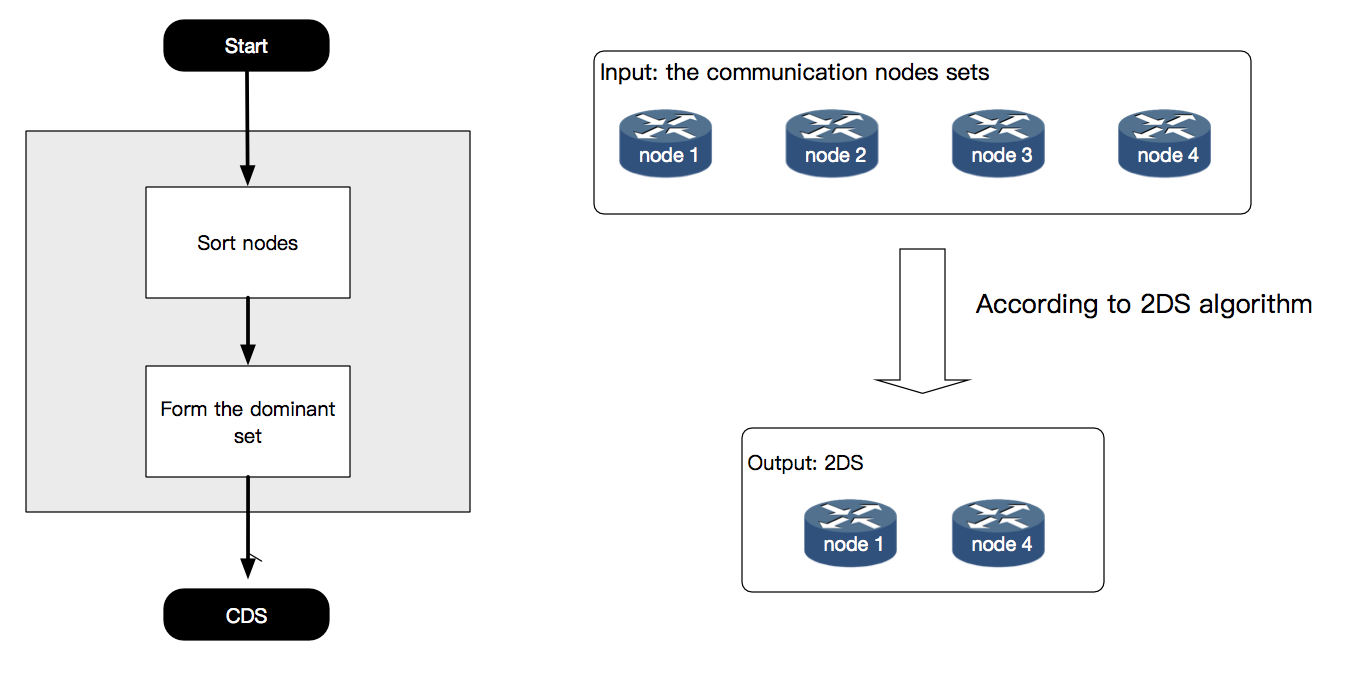
\includegraphics [width=3.5in]{A1.png}
\caption{G1}
\label{A1}
\end{figure*}

\begin{figure*}
\centering
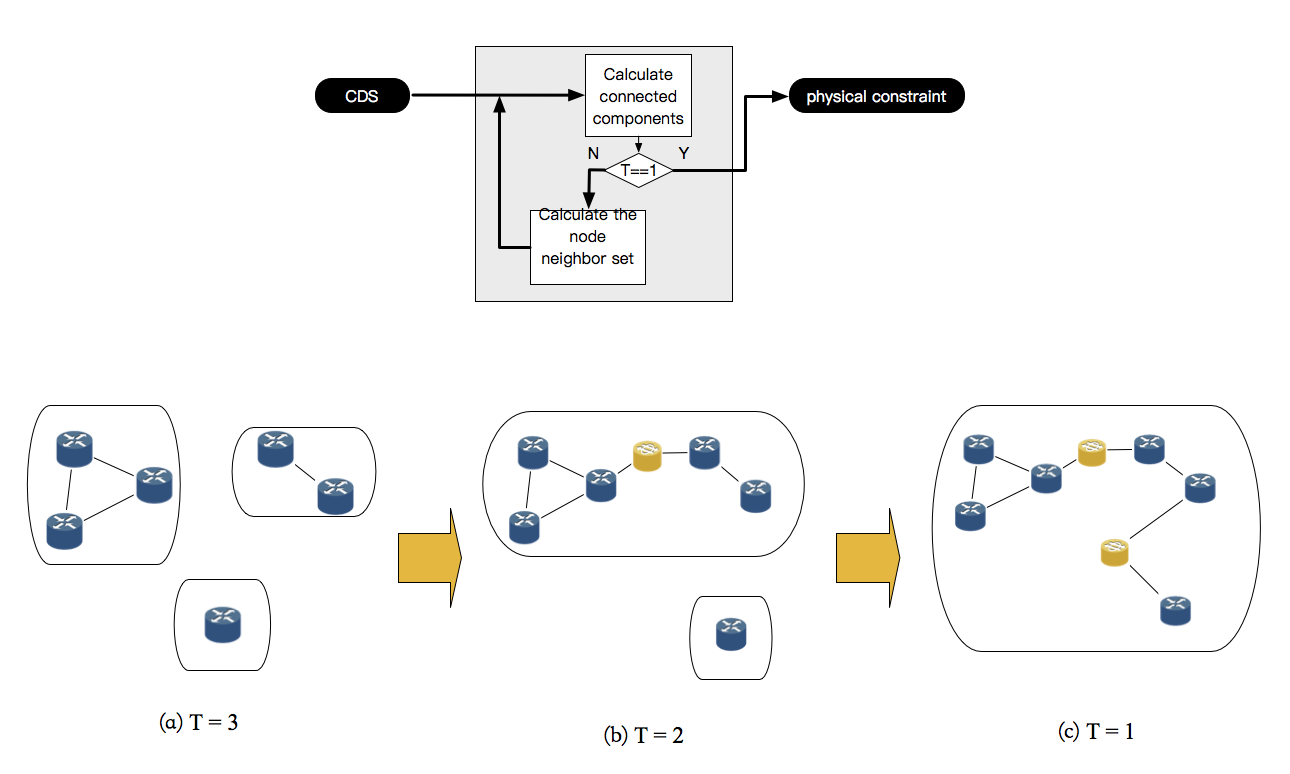
\includegraphics [width=5.5in]{A2.png}
\caption{G2}
\label{A2}
\end{figure*}




\begin{figure*}
\centering
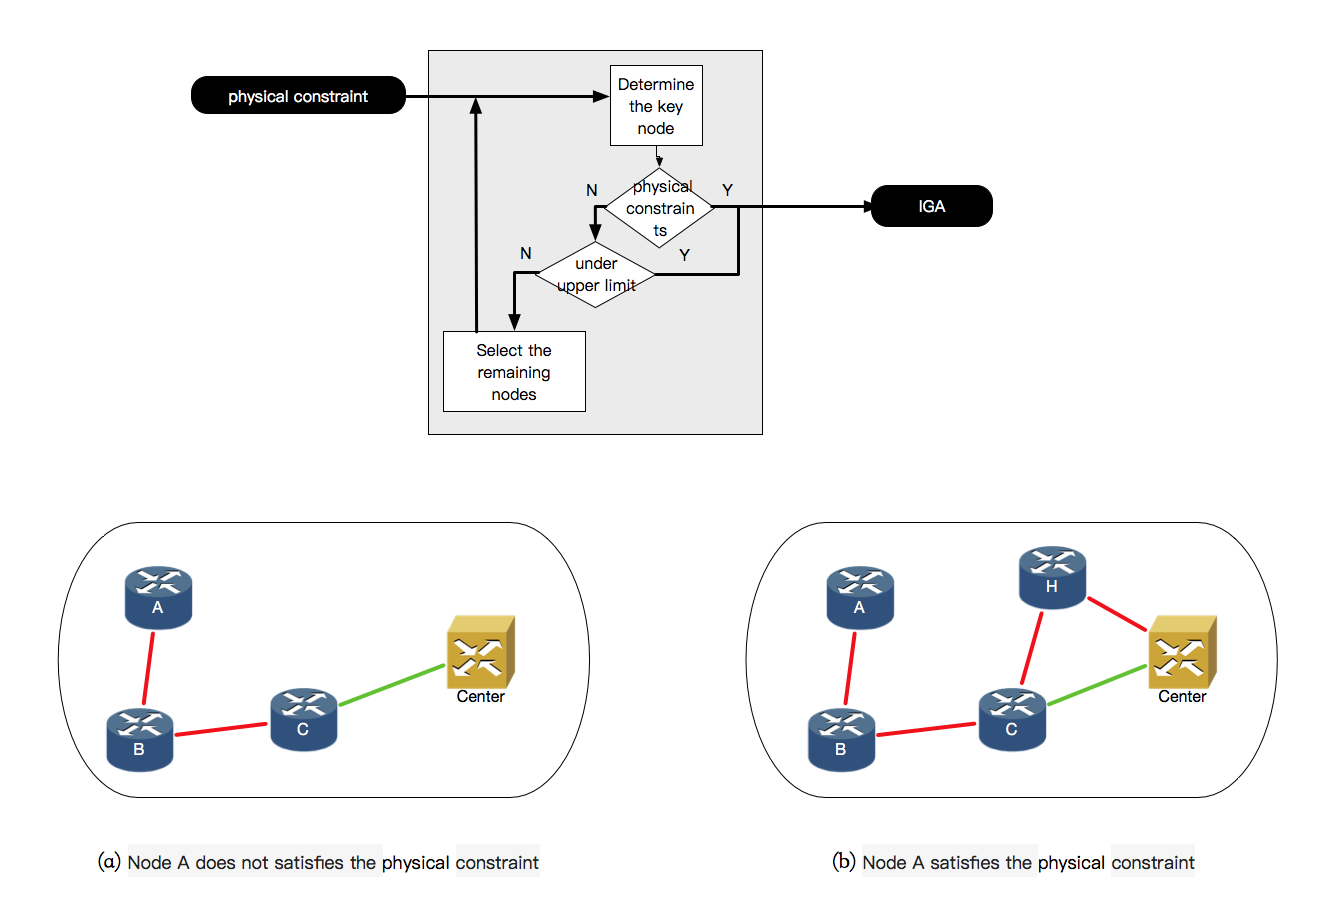
\includegraphics [width=5in]{A3.png}
\caption{Gx}
\label{A3}
\end{figure*}

\begin{figure*}
\centering
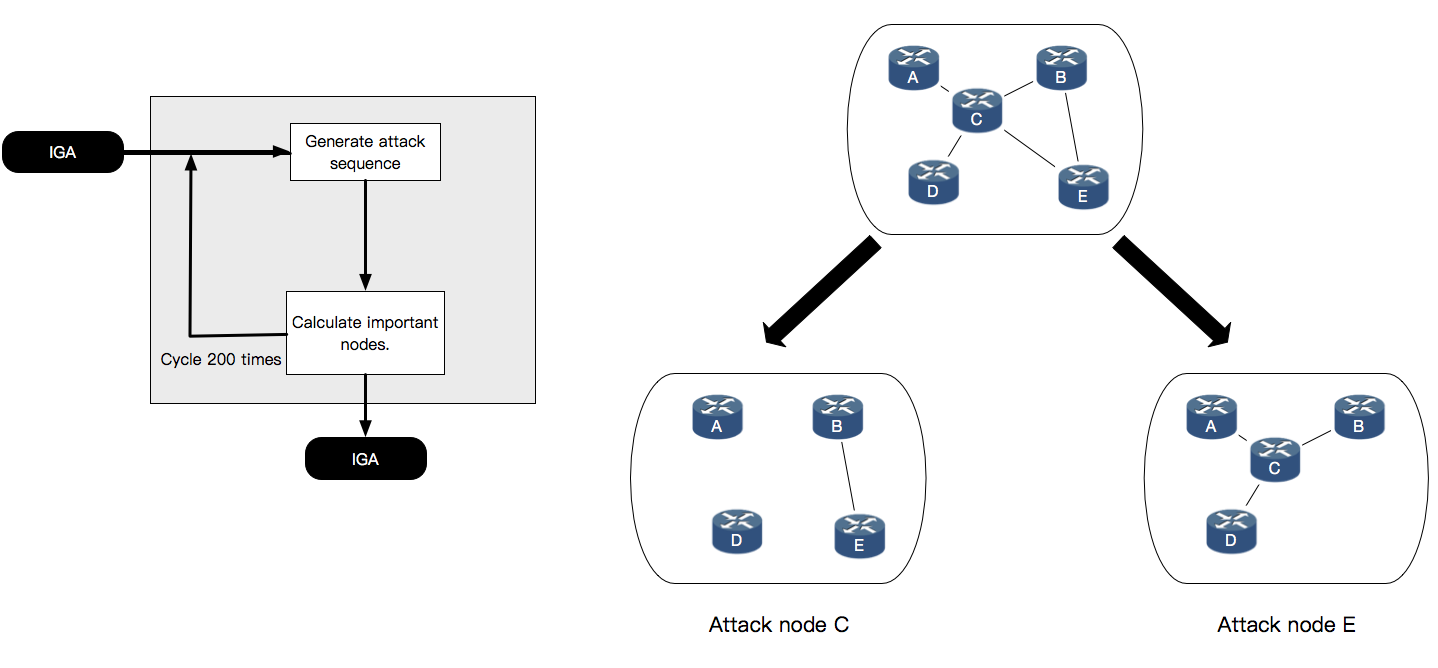
\includegraphics [width=5in]{A4.png}
\caption{Gx}
\label{A4}
\end{figure*}
\newpage
 \subsection{Time Complexity}
 \par Where the time complexity of the G1-solving algorithm is O(n\^{}2) + O(kn), and k represents the average coupling degree of the power node to the communication node. Where the time complexity of the G2-solving algorithm is O(yn\^{}2), y is the average degree of the power node network. Where the Gx-solving algorithm time complexity is O(n\^{}3), the final part differs according to the accuracy of the solution; under normal circumstances it is O(n\^{}3).
\par The average total time complexity is O(n\^{}3). If network managers use the usual sorting algorithm, the time complexity is O(n\^{}3logn). Even if this algorithm is run on a large-scale network, the user experience does not change as this algorithm runs duing the network construction period only. In the actual operation of the network, users cannot perceive any increase in time delay.

\section{Simulation experiment}
\par At present, simulation platforms for power and communication networks are still not available. This paper uses the NetworkX simulation package to generate an emulation coupled network and performs simulation experiments. NetworkX is a Python package for the creation, manipulation, and study of the structure, dynamics, and functions of complex networks [21]. The purpose of this experiment is to validate the proposed model and verify the proposed algorithm.
%\begin{comment}
\begin{figure}[htbp]
\centering                                                          %??
\subfigure[Power communication network]{                    %?????
\begin{minipage}{7cm}
\centering                                                          %????
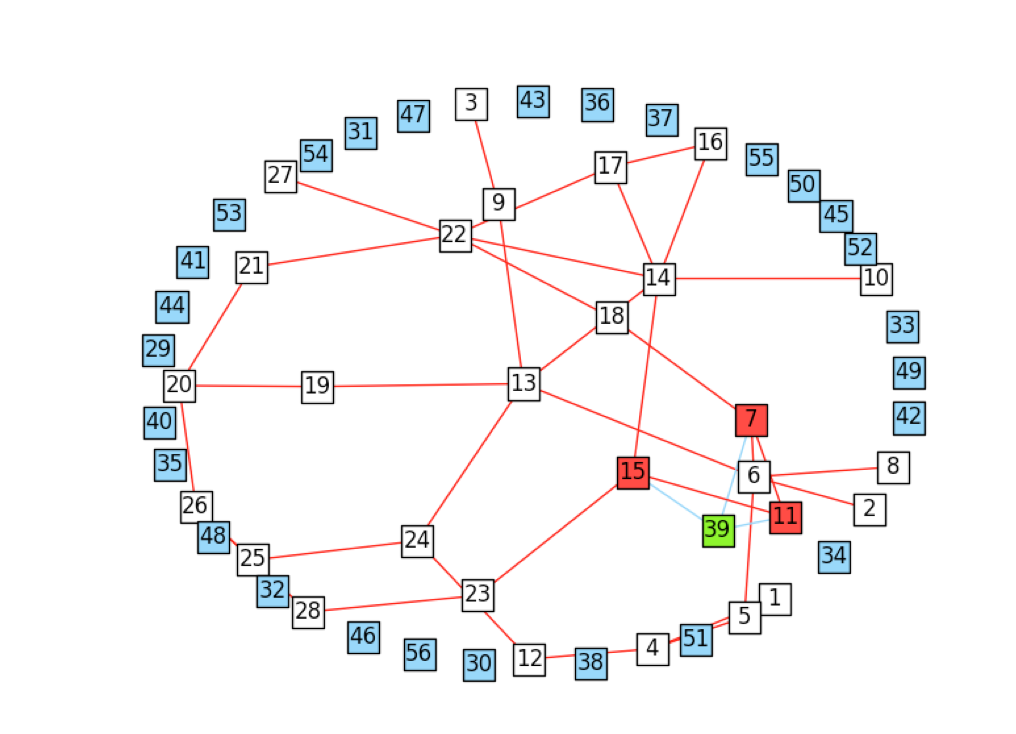
\includegraphics[scale=0.4]{9.png}               %?pic.jpg?0.5?????\
\end{minipage}}
\subfigure[Cable Network]{                    %?????
\begin{minipage}{7cm}
\centering                                                          %????
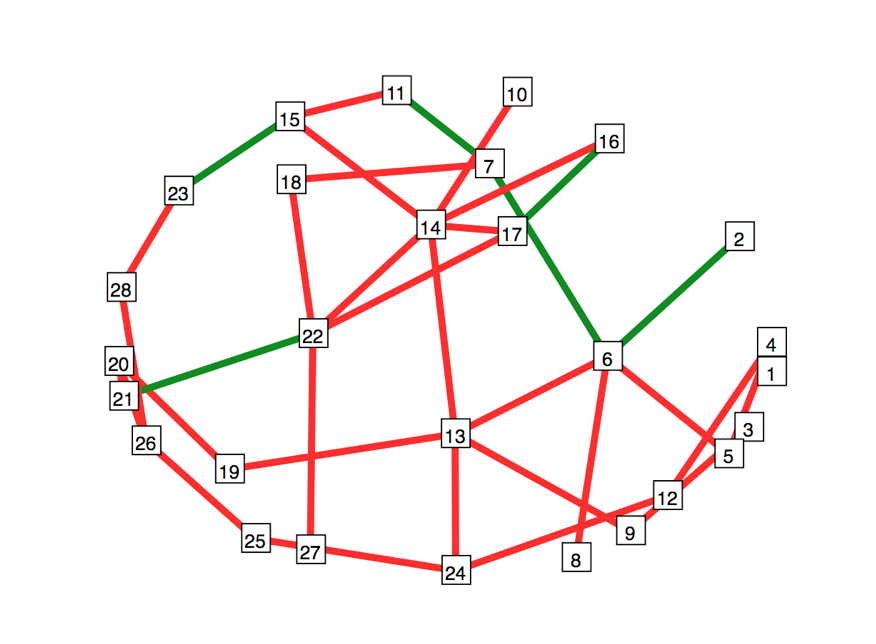
\includegraphics[scale=0.45]{11.png}                %?pic.jpg?0.5?????
\end{minipage}}
\caption{Networks} %                         %????
\label{Networks}
\end{figure}
%\end{comment} 
\par These experiments used the backbone network topology of China's three-tier power grid. We imported 28 power nodes and 28 communication nodes into NetworkX. For the convenience of analyzing the topology, we hugged most of the coupling links between the power node and the communication node in Fig. \ref{Networks} (a). Furthermore, Fig. \ref{Networks} (b) shows the different types of cables in the network. The green line indicates the O cable, and the red line indicates the A cable.


\subsection{Results}
\begin{figure}[htbp]
\centering                                                          %??
\subfigure[G1]{                    %?????
\begin{minipage}{7cm}
\centering                                                          %????
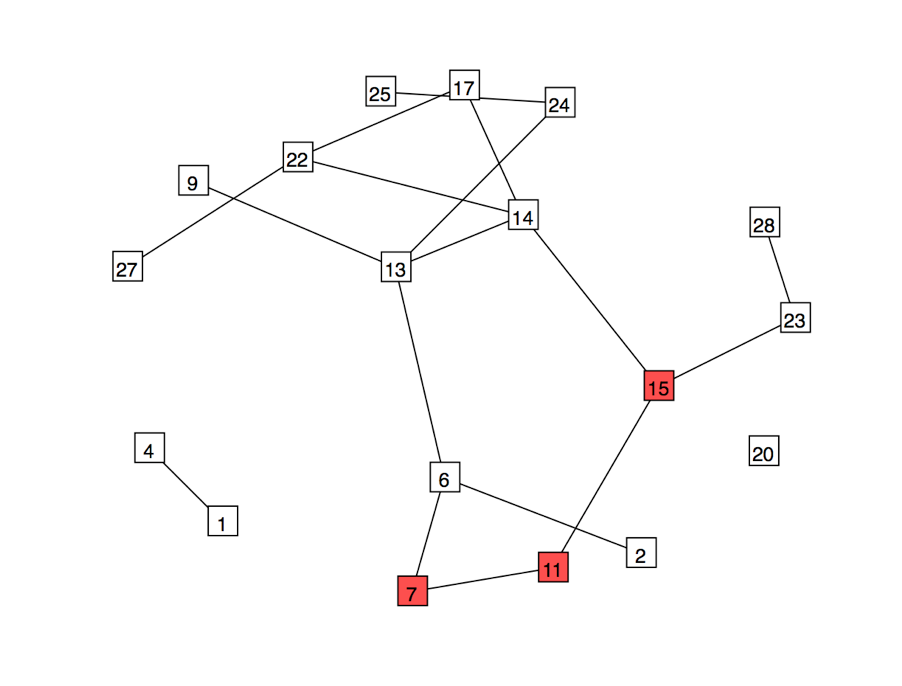
\includegraphics[scale=0.46]{13.png}               %?pic.jpg?0.5?????\
\end{minipage}}
\subfigure[G2]{                    %?????
\begin{minipage}{7cm}
\centering                                                          %????
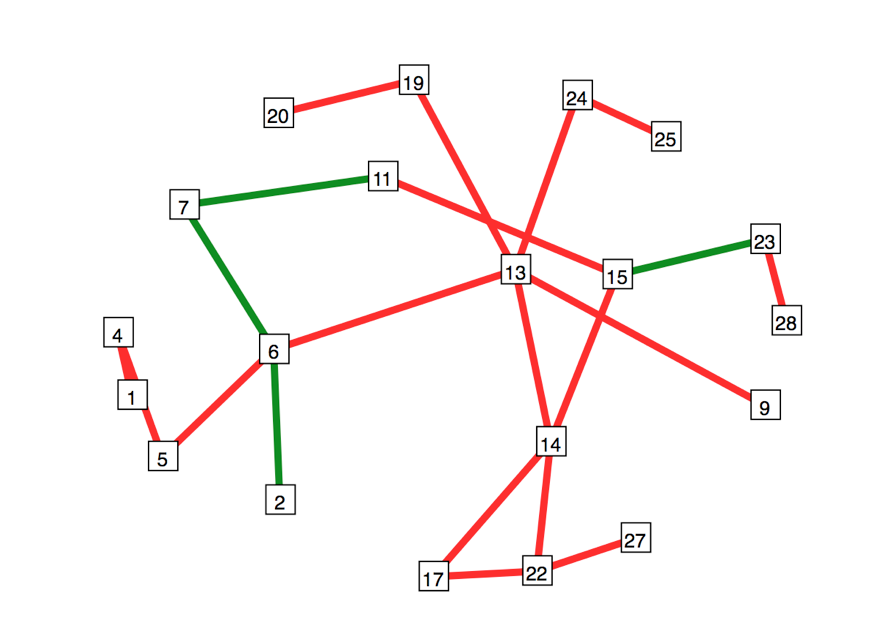
\includegraphics[scale=0.5]{15.png}                %?pic.jpg?0.5?????
\end{minipage}}
\caption{The Network Structure} %                         %????
\label{G}
\end{figure}
\par Fig. \ref{G} (a) shows the topological structure of G1. It can be seen that the dominant set is not necessarily connected. Fig. \ref{G} (b) shows the topological results of G2, and it can be seen that G2 is CDS.


%\begin{comment}

%\end{comment} 


\par The result of the Gx algorithm was G, which means that even where all nodes were added to the set, the conditions could not be satisfied. In this case, the network administrator must choose alternate methods to solve this problem, such as changing the network structure and increasing the number of cables. Here, the final result is G2.

\subsection{Fault conditions}
\begin{figure}[htbp]
\centering                                                          %??
\subfigure[Initialization]{                    %?????
\begin{minipage}{5cm}
\centering                                                          %????
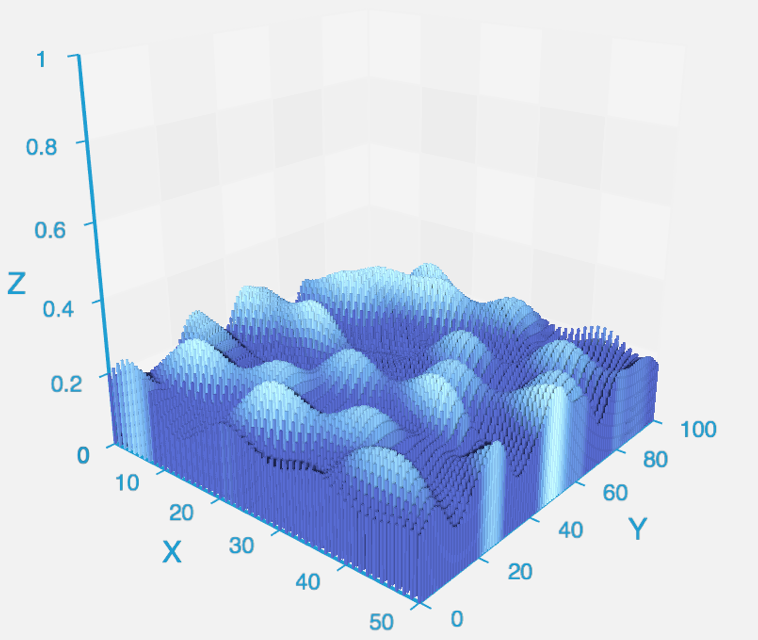
\includegraphics[scale=0.33]{21.png}               %?pic.jpg?0.5?????\
\end{minipage}}
\subfigure[PNGA]{                    %?????
\begin{minipage}{5cm}
\centering                                                          %????
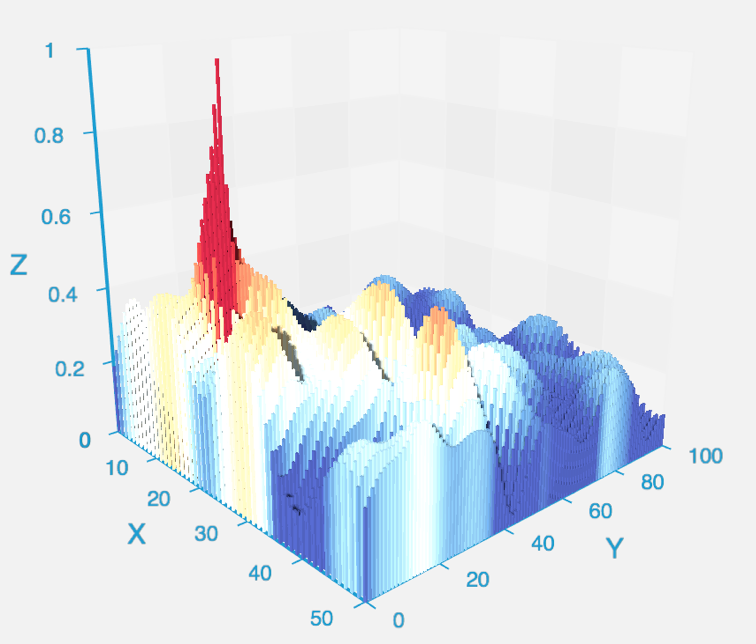
\includegraphics[scale=0.33]{22.png}                %?pic.jpg?0.5?????
\end{minipage}}
\subfigure[DSA]{                    %?3???
\begin{minipage}{5cm}
\centering                                                          %????
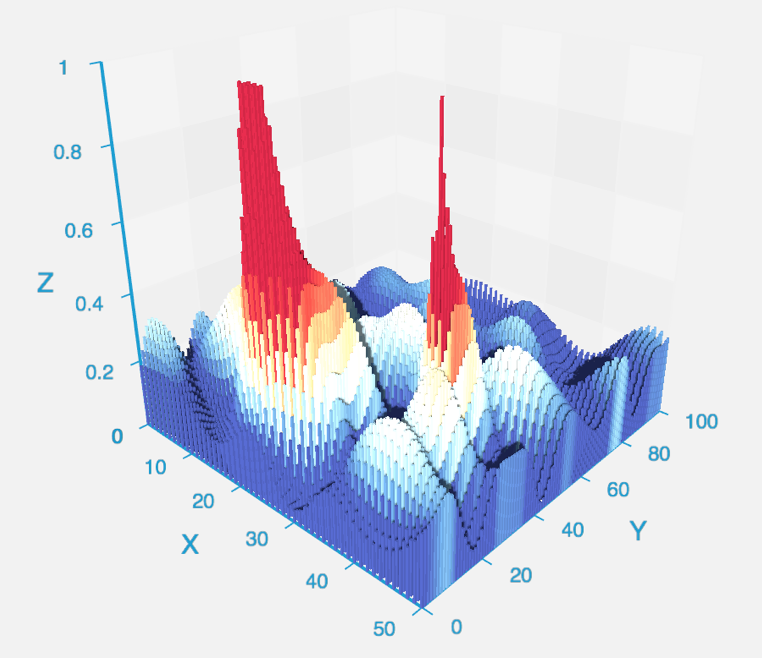
\includegraphics[scale=0.33]{23.png}               %?pic.jpg?0.5?????\
\end{minipage}}
\caption{Fault Conditions} %                         %????
\label{conditions}
\end{figure}
\par Fig. \ref{conditions} (a) shows the nodes in the initial state, and all nodes work well. We can see that DSA is inferior to PNGA from Fig. \ref{conditions} (b) and Fig. \ref{conditions} (c). The red section of the graph shows the fault rate of the nodes.


\subsection{Comparison}
\par There are two ways to attack a network: gray and black attacks. Black attacks target randomly selected nodes, which can cause a random node failures and are usually used to simulate random faults. In contrast, gray attackers understand part of the network topology. Based on this, the attacker chooses which objects to target.

\par We selected DSA and DSAS (DSA based on grid service) for the control group. The DSAS is a variant of DSA [24] that combines gird service concepts. This algorithm is superior to DSA in networks where managers focus more on grid services. The performance of the three backup strategies when black and gray failure attacks occur are shown in Fig. \ref{Fault} (a) and Fig. \ref{Fault} (b). The performance of the primitive topology (15\% of the nodes are backed up) is shown Fig. \ref{Fault} (c).
\par In the early stages of network failure attacks, the network can maintain a high rate of workable nodes. It is clear that PNGA is 10\% -15\% more effective than the other algorithms at suppressing faults during a network failure attack.
\begin{figure}[htbp]
\centering   
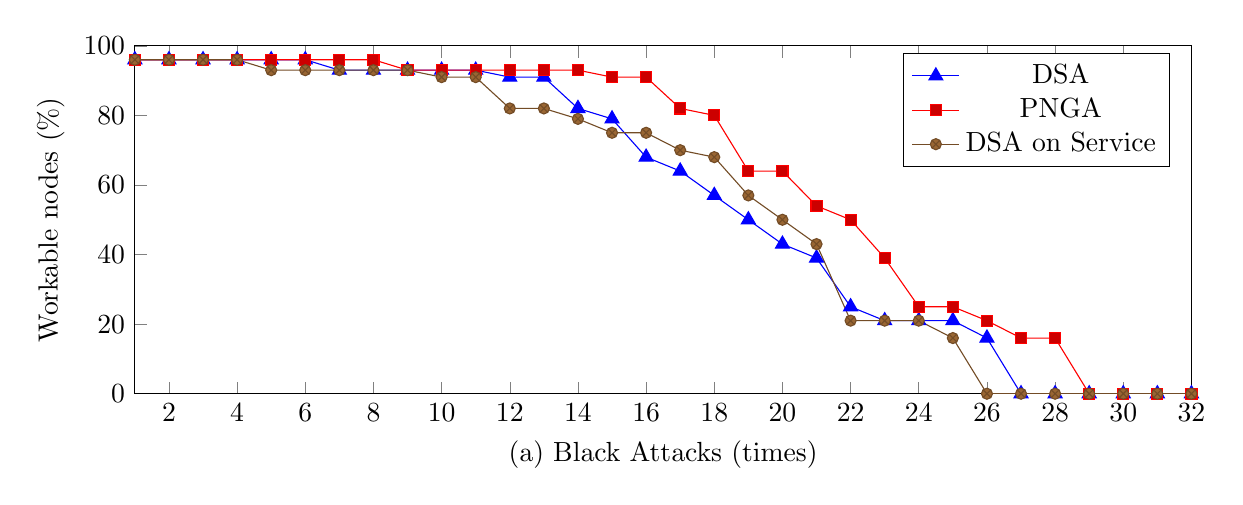
\begin{tikzpicture}
\begin{axis}
[
height=6cm,
width=15cm,
xlabel=(a) Black Attacks (times),
ylabel=Workable nodes (\%),
xmin=1,
xmax=32,
ymin=0,
ymax=100,
ytick pos=left
]
\addplot[color=blue,
    mark=triangle*, mark size=2.9pt ] coordinates {
(0,  100 )
(1,   96)
(2,   96)
(3,   96)
(4,   96)
(5,   96)
(6,   96)
(7,   93)
(8,   93)
(9,   93)
(10,   93)
(11,   93)
(12,   91)
(13,   91)
(14,   82)
(15,   79)
(16,   68)
(17,   64)
(18,   57)
(19,   50)
(20,   43)
(21,   39)
(22,   25)
(23,   21)
(24,   21)
(25,   21)
(26,   16)
(27,   0)
(28,   0)
(29,   0)
(30,   0)
(31,   0)
(32,   0)
};
\addlegendentry{DSA}

\addplot coordinates {
(0,   100 )
(1,   96)
(2,  96 )
(3,   96)
(4,   96)
(5,   96)
(6,   96)
(7,  96 )
(8,  96 )
(9,  93 )
(10, 93  )
(11,   93)
(12, 93  )
(13,  93 )
(14,  93 )
(15,  91 )
(16, 91  )
(17,  82 )
(18, 80  )
(19, 64  )
(20,  64 )
(21,  54)
(22,  50 )
(23,  39 )
(24,  25 )
(25,   25)
(26,   21)
(27,  16 )
(28,  16 )
(29,  0 )
(30,  0 )
(31,  0 )
(32,  0 )
};

\addlegendentry{PNGA}

\addplot coordinates {
(0,    100)
(1,   96)
(2,   96)
(3,   96)
(4,   96)
(5,   93)
(6,  93 )
(7,   93)
(8,   93)
(9,   93)
(10,   91)
(11,   91)
(12,   82)
(13,   82)
(14,   79)
(15,   75)
(16,   75)
(17,   70)
(18,   68)
(19,   57)
(20,   50)
(21,   43)
(22,   21)
(23,   21)
(24,   21)
(25,   16)
(26,   0)
(27,   0)
(28,   0)
(29,   0)
(30,   0)
(31,   0)
(32,   0)
};
\addlegendentry{DSA on Service}
\end{axis}
\end{tikzpicture}
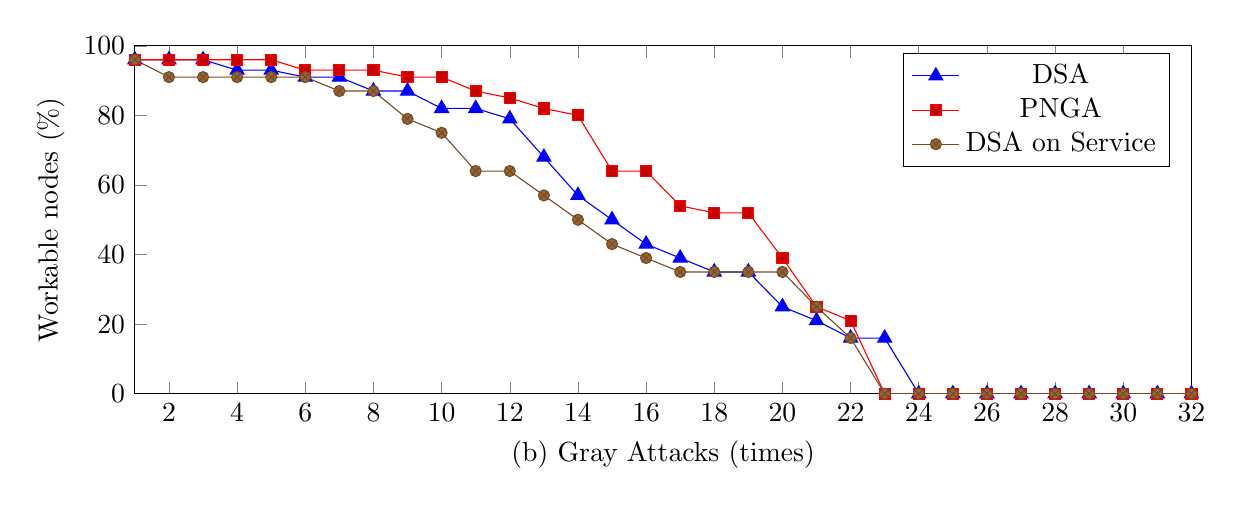
\begin{tikzpicture}
\begin{axis}
[
height=6cm,
width=15cm,
xlabel=(b) Gray Attacks (times),
ylabel=Workable nodes (\%),
xmin=1,
xmax=32,
ymin=0,
ymax=100,
ytick pos=left
]
\addplot[color=blue,
    mark=triangle*, mark size=2.9pt ]  coordinates {
(0,   100 )
(1,   96)
(2,   96)
(3,  96 )
(4,  93 )
(5,  93 )
(6,  91 )
(7,  91 )
(8,   87)
(9,   87)
(10,   82)
(11,  82 )
(12,   79)
(13,  68 )
(14,   57)
(15,   50)
(16,  43)
(17,   39)
(18,   35)
(19,  35 )
(20,   25)
(21,   21)
(22,  16 )
(23,   16)
(24,  0 )
(25,   0)
(26,   0)
(27,  0 )
(28,  0 )
(29,  0 )
(30,  0 )
(31,  0 )
(32,  0 )
};
\addlegendentry{DSA}

\addplot coordinates {
(0,   100 )
(1,   96)
(2,   96)
(3,  96 )
(4,  96 )
(5,  96 )
(6,  93 )
(7,  93 )
(8,   93)
(9,   91)
(10,   91)
(11,  87)
(12,   85)
(13,  82 )
(14,   80)
(15,   64)
(16,  64)
(17,   54)
(18,   52)
(19,  52 )
(20,   39)
(21,   25)
(22,  21 )
(23,   0)
(24,  0 )
(25,   0)
(26,   0)
(27,  0 )
(28,  0 )
(29,  0 )
(30,  0 )
(31,  0 )
(32,  0 )
};

\addlegendentry{PNGA}

\addplot coordinates {
(0,   100 )
(1,   96)
(2,   91)
(3,  91 )
(4,  91 )
(5,  91 )
(6,  91 )
(7,  87 )
(8,   87)
(9,   79)
(10,   75)
(11,  64)
(12,   64)
(13,  57 )
(14,   50)
(15,   43)
(16,  39)
(17,   35)
(18,   35)
(19,  35 )
(20,   35)
(21,   25)
(22,  16 )
(23,   0)
(24,  0 )
(25,   0)
(26,   0)
(27,  0 )
(28,  0 )
(29,  0 )
(30,  0 )
(31,  0 )
(32,  0 )
};
\addlegendentry{DSA on Service}
\end{axis}
\end{tikzpicture}

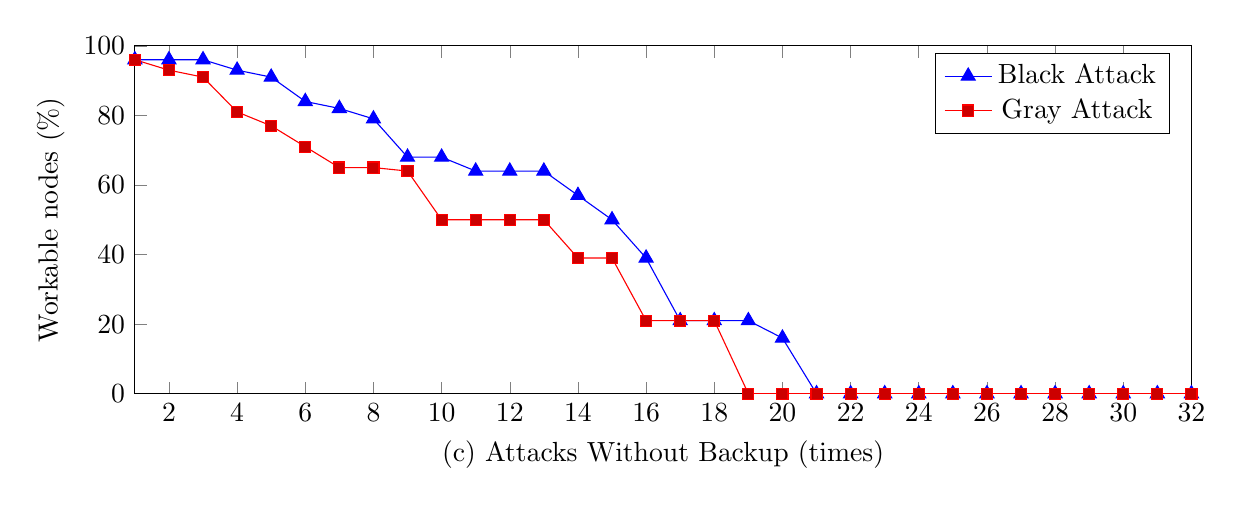
\begin{tikzpicture}
\begin{axis}
[
height=6cm,
width=15cm,
xlabel=(c) Attacks Without Backup (times),
ylabel=Workable nodes (\%),
xmin=1,
xmax=32,
ymin=0,
ymax=100,
ytick pos=left
]
\addplot[color=blue,
    mark=triangle*, mark size=2.9pt ]  coordinates {
(0,   100 )
(1,   96)
(2,   96)
(3,  96 )
(4,  93 )
(5,  91 )
(6,  84 )
(7,  82 )
(8,   79)
(9,   68)
(10,   68)
(11,  64)
(12,   64)
(13,  64 )
(14,   57)
(15,   50)
(16,  39)
(17,   21)
(18,   21)
(19,  21 )
(20,   16)
(21,   0)
(22,  0 )
(23,   0)
(24,  0 )
(25,   0)
(26,   0)
(27,  0 )
(28,  0 )
(29,  0 )
(30,  0 )
(31,  0 )
(32,  0 )

};
\addlegendentry{Black Attack}

\addplot coordinates {
(0,   100 )
(1,   96)
(2,   93)
(3,  91 )
(4,  81 )
(5,  77 )
(6,  71 )
(7,  65 )
(8,   65)
(9,   64)
(10,   50)
(11,  50)
(12,   50)
(13,  50 )
(14,   39)
(15,   39)
(16,  21)
(17,   21)
(18,   21)
(19,  0 )
(20,   0)
(21,   0)
(22,  0 )
(23,   0)
(24,  0 )
(25,   0)
(26,   0)
(27,  0 )
(28,  0 )
(29,  0 )
(30,  0 )
(31,  0 )
(32,  0 )
};

\addlegendentry{Gray Attack}

\end{axis}
\end{tikzpicture}
\caption{The Network Under Different Attacks} %                         %????
\label{Fault}
\end{figure}

\newpage


\section{Conclusion}
In this paper, we introduced the evaluation functions Q(G) and QP(G), used in Section 2, to analyze the simulation results. After sampling the results in the previous section, we obtained the charts Q(G) and QP(G), which represent the robustness of the network. 
\par Our calculations showed that the lower limit of the evaluation function was 0, which indicates that the network was extremely fragile. Furthermore, the upper limit of the evaluation function was 1, indicating that the network cannot be destroyed; specific experimental data is shown Fig. \ref{analysis}. In both attack modes, the PNGA results are superior to those of the other two algorithms. Thus, we can draw the following conclusions based on the simulation results:
\begin{itemize}
\item The node fails and the network gradually collapse as the attack progresses; however, the backup strategy can slow this process. If the attack continues, all nodes in the network cease to work.
\item Gray attacks are more devastating as attackers can choose their targets; however, after the network crashes, the two attack strategies are similar.
\item Network administrators can use this backup strategy to enhance the robustness of the network. Thus, PNGA produces superior fault suppression when compared with the other algorithms.

\end{itemize}

\begin{figure}[htbp]
\centering                                                          %??
\subfigure{                    %?????
\begin{minipage}{8.5cm}

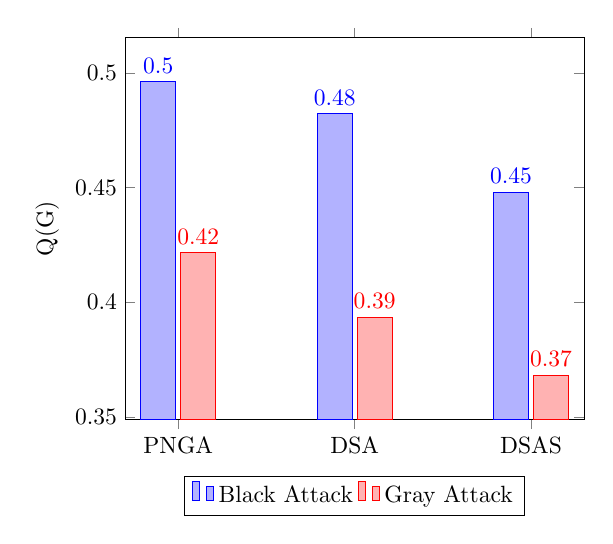
\begin{tikzpicture}[scale=0.85]
\begin{axis}[
    ybar,
    enlargelimits=0.15,
    legend style={at={(0.5,-0.15)},
      anchor=north,legend columns=-1},
    ylabel={Q(G)},
    symbolic x coords={PNGA,DSA,DSAS},
    xtick=data,
    nodes near coords,
    nodes near coords align={vertical},
    bar width=15pt,
    ]
\addplot coordinates {(PNGA,0.49616) (DSA,0.48234) (DSAS,0.44813)};
\addplot coordinates {(PNGA,0.42171) (DSA,0.39348) (DSAS,0.36827)};
\legend{Black Attack,Gray Attack}
\end{axis}
\end{tikzpicture}
\end{minipage}}
\subfigure{                    %?????
\begin{minipage}{8.5cm}
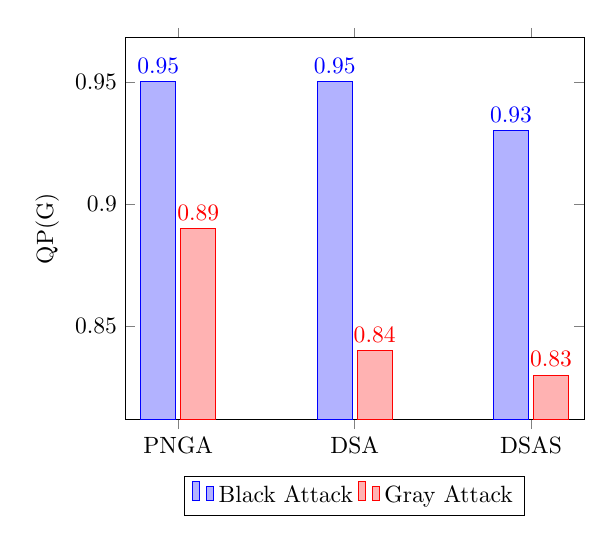
\begin{tikzpicture}[scale=0.85]
\begin{axis}[
    ybar,
    enlargelimits=0.15,
    legend style={at={(0.5,-0.15)},
      anchor=north,legend columns=-1},
    ylabel={QP(G)},
    symbolic x coords={PNGA,DSA,DSAS},
    xtick=data,
    nodes near coords,
    nodes near coords align={vertical},
    bar width=15pt,
    ]
\addplot coordinates {(PNGA,0.95) (DSA,0.95) (DSAS,0.93)};
\addplot coordinates {(PNGA,0.89) (DSA,0.84) (DSAS,0.83)};
\legend{Black Attack,Gray Attack}
\end{axis}
\end{tikzpicture}

\end{minipage}}
\caption{Analysis} %                         %????
\label{analysis}
\end{figure}
\par There are some conditions that this article does not consider. For example, evaluating the efficacy of 2-CDS in a real-world environment, how to extend the heuristic algorithm proposed in this paper to the other MCDS problems and whether the optical cables in the power communication network has other effects on the fault suppression. These questions will guide our subsequent research.
% An example of a floating figure using the graphicx package.
% Note that \label must occur AFTER (or within) \caption.
% For figures, caption should occur after the \includegraphics.
% Note that IEEEtran v1.7 and later has special internal code that
% is designed to preserve the operation of \label within \caption
% even when the captionsoff option is in effect. However, because
% of issues like this, it may be the safest practice to put all your
% \label just after \caption rather than within \caption{}.
%
% Reminder: the "draftcls" or "draftclsnofoot", not "draft", class
% option should be used if it is desired that the figures are to be
% displayed while in draft mode.
%
%\begin{figure}[!t]
%\centering
%\includegraphics[width=2.5in]{myfigure}
% where an .eps filename suffix will be assumed under latex, 
% and a .pdf suffix will be assumed for pdflatex; or what has been declared
% via \DeclareGraphicsExtensions.
%\caption{Simulation results for the network.}
%\label{fig_sim}
%\end{figure}

% Note that the IEEE typically puts floats only at the top, even when this
% results in a large percentage of a column being occupied by floats.


% An example of a double column floating figure using two subfigures.
% (The subfig.sty package must be loaded for this to work.)
% The subfigure \label commands are set within each subfloat command,
% and the \label for the overall figure must come after \caption.
% \hfil is used as a separator to get equal spacing.
% Watch out that the combined width of all the subfigures on a 
% line do not exceed the text width or a line break will occur.
%
%\begin{figure*}[!t]
%\centering
%\subfloat[Case I]{\includegraphics[width=2.5in]{box}%
%\label{fig_first_case}}
%\hfil
%\subfloat[Case II]{\includegraphics[width=2.5in]{box}%
%\label{fig_second_case}}
%\caption{Simulation results for the network.}
%\label{fig_sim}
%\end{figure*}
%
% Note that often IEEE papers with subfigures do not employ subfigure
% captions (using the optional argument to \subfloat[]), but instead will
% reference/describe all of them (a), (b), etc., within the main caption.
% Be aware that for subfig.sty to generate the (a), (b), etc., subfigure
% labels, the optional argument to \subfloat must be present. If a
% subcaption is not desired, just leave its contents blank,
% e.g., \subfloat[].


% An example of a floating table. Note that, for IEEE style tables, the
% \caption command should come BEFORE the table and, given that table
% captions serve much like titles, are usually capitalized except for words
% such as a, an, and, as, at, but, by, for, in, nor, of, on, or, the, to
% and up, which are usually not capitalized unless they are the first or
% last word of the caption. Table text will default to \footnotesize as
% the IEEE normally uses this smaller font for tables.
% The \label must come after \caption as always.
%
%\begin{table}[!t]
%% increase table row spacing, adjust to taste
%\renewcommand{\arraystretch}{1.3}
% if using array.sty, it might be a good idea to tweak the value of
% \extrarowheight as needed to properly center the text within the cells
%\caption{An Example of a Table}
%\label{table_example}
%\centering
%% Some packages, such as MDW tools, offer better commands for making tables
%% than the plain LaTeX2e tabular which is used here.
%\begin{tabular}{|c||c|}
%\hline
%One & Two\\
%\hline
%Three & Four\\
%\hline
%\end{tabular}
%\end{table}


% Note that the IEEE does not put floats in the very first column
% - or typically anywhere on the first page for that matter. Also,
% in-text middle ("here") positioning is typically not used, but it
% is allowed and encouraged for Computer Society conferences (but
% not Computer Society journals). Most IEEE journals/conferences use
% top floats exclusively. 
% Note that, LaTeX2e, unlike IEEE journals/conferences, places
% footnotes above bottom floats. This can be corrected via the
% \fnbelowfloat command of the stfloats package.


\section*{Acknowledgment}

The work presented in this paper was supported by the National Natural Science Foundation of China (61302078, 61372108), 863 Program (2011AA01A102), National S\&T Major Project (2011ZX 03005-004-02).

\begin{thebibliography}{1}

\bibitem{IEEEhowto:kopka}
 Ye Y, et al. A Survey on Smart Grid Communication Infrastructures: Motivations, Requirements and Challenges, IEEE Communications Surveys Tutorials, 2013, 15(1):5-20.

\bibitem{IEEEhowto:kopka}
Jingchen Gao, et al. A survey of communication networking in Smart Grids, Future Generation Computer Systems, 2012, 28:391-404.
\bibitem{IEEEhowto:kopka}
Ancillotti E, et al. The role of communication systems in smart grids: architectures, technical solutions and research challenges, Computer Communications, 2013, 36 (17-18):1665-1697. 
 \bibitem{IEEEhowto:kopka}
Gungor V C, et al. A Survey on Smart Grid Potential Applications and Communication Requirements , IEEE Transactions on Industrial Informatics. 2013, 9(1):28-42.
  \bibitem{IEEEhowto:kopka}
Serizawa Y, et al. Present and Future ICT Infrastructures for a Smarter Grid in Japan, 2010 IEEE Innovative Smart Grid Technologies (ISGT), Gaithersburg, 2010:1-5.
    \bibitem{IEEEhowto:kopka}
Milioudis A N, et al. Detection and Location of High Impedance Faults in Multi-conductor Overhead Distribution Lines Using Power Line Communication Devices, IEEE Transactions on Smart Grid, 2015, 6(2):894-902.

\bibitem{IEEEhowto:kopka}
R. Mijumbi, et al. Network Function Virtualization: State-of-the-Art and Research Challenges, IEEE Communications Surveys Tutorials, vol. 18, no. 1, pp. 236-262, Firstquarter 2016.

\bibitem{IEEEhowto:kopka}
Xiang Cheng, et al. Virtual network embedding through topology-aware node ranking. ACM SIGCOMM Computer Communication Review. 2011
\bibitem{IEEEhowto:kopka}
Subharthi Paul, et al. Architectures for the future networks and the next generation Internet: A survey. Computer Communications. 2010 
\bibitem{IEEEhowto:kopka}
 Andreas Berl, et al. Virtualisierung im Future Internet. Informatik-Spektrum. 2010

\bibitem{IEEEhowto:kopka}
Ze Shao, et al. A network risk assessment methodology for power communication business. 2016 IEEE International Conference on Network Infrastructure and Digital Content (IC-NIDC).
\bibitem{IEEEhowto:kopka}
Liu Xintong, et al. The implementation and application of security evaluation system of Electric Power Communication Network.  2016 2nd IEEE International Conference on Computer and Communications (ICCC).



\bibitem{IEEEhowto:kopka} Jiang Z, et al. Enhancing network performance by edge addition International Journal of Modern Physics C 2011 22 11:1211-1226.
\bibitem{IEEEhowto:kopka}
Topological Vulnerability Analysis and Countermeasures of Electrical Communication Network Based on Complex Network Theory Power System Technology 2015:12.
\bibitem{IEEEhowto:kopka} Zhou Jing, et al. Study on bandwidth analysis and capacity planning of provincial dispatching digital network, Power System Technology 2012,36(5):173-177.


\bibitem{IEEEhowto:kopka}
D. Kim, X, et al. Construction of Fault-Tolerant Virtual Backbones in Wireless Networks, Handbook on Security and Networks, World Scientific Publishing (edited by Y. Xiao, F.H. Li, and H. Chen), pp. 488-509, April 2011.
\bibitem{IEEEhowto:kopka}
H. Du, et al. Connected Dominating Set in Wireless Networks, to appear in Handbook of Combinatorial Optimization, Springer (edited by P.M. Pardalos, D.-Z. Du, and R. Graham), July 2013.


\bibitem{IEEEhowto:kopka}
 Jianyuan Feng, et al. An Approach to 5G Wireless Network Virtualization: Architecture and Trial Environment. 2017 IEEE Wireless Communications and Networking Conference (WCNC) Year: 2017





                                
\bibitem{IEEEhowto:kopka}
Yu Q. Applications of Flexible AC Transmissions System (FACTS) Technology in Smart Grid and its EMC Impact, 2014 IEEE International Symposium on Electromagnetic Compatibility (EMC), Raleigh, 2014:392-397.
\bibitem{IEEEhowto:kopka}
Falahati B, F Yong. Reliability Assessment of Smart Grids Considering Indirect Cyber-Power Interdependencies, IEEE Transaction on Smart Grid, 2014, 5(4):1677-1685.
\bibitem{IEEEhowto:kopka}
Dong-Hoon S, Q Dajun, Z Junshan, Cascading Effects in Interdependent Networks , IEEE Network, 2014, 28(4):82-87.


\bibitem{IEEEhowto:kopka}
Yunfei Guo, et al.Research on reliability evaluation model and path optimization for power communication network. 2015 5th International Conference on Electric Utility Deregulation and Restructuring and Power Technologies (DRPT).
\bibitem{IEEEhowto:kopka}
Shi Jian, et al. Research on reliability evaluation of power communication network. 2014 International Conference on Power System Technology.

\bibitem{IEEEhowto:kopka}
 Arun Das, et al. Root Cause Analysis of Failures in Interdependent Power-Communication Networks. 2014 IEEE Military Communications Conference.

\bibitem{IEEEhowto:kopka}
Jinghong Guo. Study on the structure of electric power communication network of strong and Smart Grid in China. 2010 International Conference on Power System Technology.
\bibitem{IEEEhowto:kopka}
 Li Jie, et al. Analysis of Power Grid Control Service Information and Communication Network Reliability Model. 2010 Second International Conference on Modeling, Simulation and Visualization Methods.
\bibitem{IEEEhowto:kopka}
Hanene Ben Yedder, et al. Trajkovic. Comparison of Virtualization Algorithms and Topologies for Data Center Networks. 2017 26th International Conference on Computer Communication and Networks (ICCCN).
\bibitem{IEEEhowto:kopka}
Omer Narmanlioglu; Engin Zeydan. Network virtualization for Mobile Operators in Software-Defined based LTE networks. 2017 IFIP/IEEE Symposium on Integrated Network and Service Management (IM).

\bibitem{IEEEhowto:kopka}Ma Chen, et al. Active monitoring service based multi-link failure location algorithm for electric power optical transport networks, Power System Technology,2013,37(11):3221-3226.

\bibitem{IEEEhowto:kopka}
Ningzhe Xing, et al. Load balancing-based routing optimization mechanism for power communication networks.

\bibitem{IEEEhowto:kopka} Zhou Jing, et al.A network optimization method based on resource sharing of power optical cable lines, Power System Technology,2011, 35(5):199-203.




 \end{thebibliography}

\newpage
 
\begin{appendix}  
\section{G1-Solving Algorithm}  
\begin{CJK*}{UTF8}{gkai}
    \begin{algorithm}
        \begin{algorithmic}[1] %??????
            \Require G
            \Ensure  G1
       
            \Function {G1-Solving}{$G$}
              
                \State $ArrayVp\gets G.Vp$
                \State $ArrayVc\gets G.Vc$
                \State $ArrayEpc<Vp,Vc>\gets G.Epc$   
                \State $ArrayEcc<Vc,Vc>\gets G.Ecc$ 

                \State $G1\gets 0$
                \State $i\gets 0$
                
                \While{$i<MapVpc.Length-1$}
                    \State $ArrayNeigh \gets MapVpc[i].value$
                    \State $length \gets ArrayNeigh.length$
                    \If{$length == 1$ \textbf{or} $length == 2$}
                        \State $G1.add(ArrayNeigh)$
                    \Else   
                    	\State $lack\gets ArrayNeigh \cup G1$
			\If{$lack== 1$ \textbf{or} $lack == 0$}
                        		\State $G1.add(MapVcc.getBySort(2-lack))$
                  	\EndIf
                    \EndIf
                \EndWhile
                 \State \Return{$G1$}
            \EndFunction
            
        \end{algorithmic}
    \end{algorithm}
\end{CJK*}
\newpage
\section{G2-Solving Algorithm}  
\begin{CJK*}{UTF8}{gkai}
    \begin{algorithm}
        \begin{algorithmic}[1] %??????
            \Require G1
            \Ensure G2
            \State \textbf{global} $ArrayState\gets 0$
            \State \textbf{global} $T\gets 1$
             \State \textbf{global} $MapN<k,Vc>$
            \Function {G2-Solving}{$G1$}
              
                \State $G2\gets G1$
                \State $ArrayN\gets 0$
                \State $\Call{ConnectSubGragh}{$G$} $
	        \State $i\gets 0$
                \While{$T>=2$}
                    \State $node \gets MapN.getFirst(i)$
                    \State $\Call{ResetGraph}{$node$}$
                    \State $G2.add(node)$
                    \State $\Call{ResetMapN}{$MapVcc)$}$
                \EndWhile
                 \State \Return{$G2$}
            \EndFunction
            \Function {ResetMapN}{$MapVcc$}
            	 \For{$<Vc,ArrayNeighVc>:MapVcc$}
			\If{$ArrayState[Vc]==0$}
				\State $MapN.add(ArrayState[ArrayNeighVc])$
			\EndIf
		\EndFor            
            \EndFunction
        \end{algorithmic}
    \end{algorithm}
    \end{CJK*}
\newpage
    
\section{Gx-Solving Algorithm}  
 \begin{algorithm}
        \begin{algorithmic}[1] %??????
            \Require G2
            \Ensure Gx
            \State \textbf{global} $ArrayEdge\gets 0$

            \Function {Gx-Solving}{$G2$}
               \State $T\gets False$
                \State $ArrayEnd\gets ArrayVc.getPower()$
                 \State $NodeLeft\gets ArrayVc - G2$
                 \State $G2.append(ArrayEnd)$
                 \State $Gx \gets G2$
                \While{\textbf{not} $T$}
                    \For {each $node \in ArrayEnd$}
                     	\State $ArrayPath\gets 0$
                    	\State $ArrayPath.append(Shortest(G2, node))$
	 	  \EndFor
		\If{$Type$  \textbf{in}  $each$ $path \in ArrayPath$}
                        	\For {each $path \in ArrayPath$}
				 \If{$DifferentType  \in$ path}
					\State $ArrayPath[path.Type]]++$
				 \EndIf
		   	\EndFor
		\EndIf
 		\State $ T \gets  max(ArrayPath) == 0$
		\If{$NodeLeft ==  \emptyset $}
                        $ T \gets True $
		\EndIf
		\If{\textbf{not}  $T$}
                      \State $ Gx.append(max(NodeLeft)) $
		\EndIf
                \EndWhile
                 \State \Return{$Gx$}
            \EndFunction
        \end{algorithmic}
    \end{algorithm}
\end{appendix} 
\end{document}




